\chapter{RPGLite: A System to Model}\label{chap:rpglite}

\inline{Ensure a consistent tense is used throughout}

To investigate whether models can be augmented using \aop{}, \pdsfthree{} can be
employed to produce \aspectoriented{} models --- but a system to model is
required. To address the research questions introduced in \cref{subsec:rqs}, a
system is required which can be modelled, and for which the accuracy of that
model's representation of the system can be measured. This is required because
the aspectually augmented model must be compared to the model without aspects
woven to discern which is more accurate. This chapter introduces a suitable
system, RPGLite, a game for which play can be modelled simply and augmented
using \aop{}. RPGLite was implemented and deployed on iOS and Android to collect
real-world play data to compare simulation output against. Techniques for
performing these comparisons are introduced in \cref{chap:experiment_setup} and
the results of these comparisons are presented in
\cref{chap:experimental_results}. This chapter describes the design of RPGLite,
its implementation as a mobile game, and the data collected from its use.

RPGLite is a game designed to mimic existing popular games, while being
structured to permit exploring all game states via formal methods.
\citet{kavanagh2020} have produced formal models using a model-checker, PRISM,
which identifies optimal play strategies in all states a game can
reach.\footnote{Game states are explained in \cref{rpglite_game_states}.} Some
experiments were conducted using RPGLite by \citet{kavanagh2021thesis} to
investigate whether players' interactions with the game converged on optimal
play.

RPGLite gameplay data invites many research questions.
\citeauthor{kavanagh2020}'s original RPGLite design as a formal model was
intended to allow the calculation of the \emph{``cost''} of an
action~\cite{kavanagh2020,kavanagh2021thesis} (the degree to which a player is
less likely to win having made a given move instead of the optimal one),
allowing for rich analysis of gameplay datasets. However, another possibility
invited by these datasets is that they enable the development of models of
individuals' gameplay. This offers an opportunity to investigate the
effectiveness of aspect-oriented simulation and modelling: the style of play of
different individuals may be best encoded by different advice (or parameters for
that advice).

RPGLite is of interest in other ways than the study of gameplay and game design.
The game is a \sociotechnical system which can produce useful datasets to
support multiple avenues of research in different disciplines. \footnote{Later
contributions in this thesis are supported by datasets produced by RPGLite, as
were the contributions of \citeauthor{kavanagh2021thesis}'s PhD
thesis~\cite{kavanagh2021thesis}. } A dataset of real-world RPGLite play would
support future work in a variety of fields as a non-commercial dataset for
research, including at least game design and gameplay
research~\cite{kavanagh2021thesis}, formal methods~\cite{kavanagh2020},
sociotechnical simulation \& modelling research as in the following chapters,
and research software engineering tooling demonstration also in the following
chapters.

For this reason, this research includes a collaboration with
\citeauthor{kavanagh2021thesis} to develop and release a mobile implementation
of RPGLite which collects gameplay data for research purposes. This dataset
enabled \citeauthor{kavanagh2021thesis} to demonstrate the utility of their
model checking in an empirical scenario~\cite{kavanagh2021thesis}. With regards
the research presented in later chapters it enables the analysis of models
representing player behaviour. The mobile game contributes this by supporting
the comparison of these models' output against the collected data, and providing
the basis of a model which can be augmented using \aop{}. The model, introduced
in \cref{chap:experiment_setup}, represents random play. Aspects are written
which augment the model to better represent real-world play, the results of
which are presented in \cref{chap:experimental_results}. If the aspectually
augmented models generate gameplay data which correlates with empirically
sourced data more closely than that generated by the unmodified model, we can
dismiss unmodified play as ``unrealistic'', and understand the aspectually
augmented behaviour as ``more realistic'' --- however, the mobile game is
required to provide the real-world data enabling this comparison.

This chapter focuses only on the design of RPGLite, its implementation as a
mobile game, and the dataset collected from real-world
play~\cite{RPGLiteLessonsLearned}. It starts with an overview of RPGLite itself
in \cref{sec:rpglite_overview}, and progresses to discuss the game's
implementation in \cref{sec:rpglite_implementation} including an application for
iOS and Android (\cref{rpglite_mobile_app}), the server and API powering its
online functionality (\cref{subsec:server-side-logic}), and the recruitment of
players to use the game (\cref{subsec:consent_to_participation}). Some insights
from the game development process are given in
\cref{rpglite_lessons_learned_summary}, which summarises already-published
contributions~\cite{RPGLiteLessonsLearned}. The game's multiple configurations
are described in are described in \cref{seasons_of_rpglite} followed by a
description of the dataset produced by players of the game in
\cref{sec:rpglite_data_discussed} before the chapter concludes with a brief
summary (\cref{rpglite_discussion_section}).

\section{An Overview of RPGLite}
\label{sec:rpglite_overview}

RPGLite is a two-player game and is played in turns. Each player selects two
characters to play with independently of their opponent. Each character has a
unique set of abilities and properties, which are health, chance of success on
attack, and damage dealt on a successful attack as well as special abilities and
properties for some characters. Eight characters are available for selection.
Characters are differentiated by the special effect they may use when attacking
an opponent character. They are defined alongside their special abilities in
\cref{fig:chars_and_their_abilities}. Specific parameters for each character ---
their health, chance to hit, and damage on hit as well as character-specific
details depending on their special abilities --- are defined as a
\emph{``configuration''} of RPGLite. Two configurations were released as
different \emph{``seasons''} of the RPGLite mobile game, which are discussed in
\cref{rpglite_configurations}.

\begin{table}
  \centering
\begin{tabular}{@{}lp{0.65\columnwidth}@{}}
  \toprule{}
  \emph{Character} & \emph{Special Ability when Attacking}\\
  \midrule{}
  Knight & Deals damage to an opponent character on a successful
  hit \tabularnewline{} 
  \rule{0pt}{2em}Archer & Deals damage to two opponent
  characters on a successful hit \tabularnewline{} 
  \rule{0pt}{2em}Wizard &
  Deals damage to an opponent character on a successful hit, disabling (or
  \emph{``stunning''}) them for the duration of the opponent's next
  turn\tabularnewline{} 
  \rule{0pt}{2em}Healer & Deals damage to an opponent
  character on a successful hit, and heals themselves or, optionally, the other
  player character instead (assuming that character is still
  alive)\tabularnewline{} 
  \rule{0pt}{2em}Barbarian & Deals damage to an opponent
  character on a successful hit, dealing additional damage if their own health
  is low when attacking\tabularnewline{} 
  \rule{0pt}{2em}Rogue & Deals damage to
  an opponent character on a successful hit, dealing additional damage if the
  target's health is low when attacked\tabularnewline{} 
  \rule{0pt}{2em}Monk &
  Deals damage to an opponent character on a successful hit, and immediately
  takes another turn, until their attack is unsuccessful\tabularnewline{}
  \rule{0pt}{2em}Gunner & Deals damage to an opponent regardless of success,
  dealing additional damage on a successful hit\\
\bottomrule{}
\end{tabular}
\caption{RPGLite characters and their unique special abilities.}
\label{fig:chars_and_their_abilities}
\end{table}

To act on their turn, each player selects an
``alive'' character (one with health greater than 0) to attach a chosen
``alive'' target of their opponent, with caveats for some characters' special
abilities. A successful attack is randomly determined by the chance of a
successful attack for the character selected by the active player. If
successful, the attack deals damage, and also results in that character's unique
ability being activated. When starting a game, a random player is chosen to take
a first move. Players may always skip their turn as a valid action. Players
continue to take alternating turns until one player has no ``alive'' characters.
They lose, and their opponent is the victor.

Different configurations change the game's \emph{``balance''}, a term referring
to the relative strengths of different characters or character pairs. For
example, if a configuration leaves many characters with initial health values
close to a Barbarian's threshold for additional damage, then they become a very
powerful character due to their ability to inflict additional damage. If the
Monk's chance to hit is high, the repeated turns it offers can be very
advantageous. Character skills can work in concert with each other: choosing a
Barbarian and Healer such that the barbarian can be kept at low health for
additional damage, but the healer can be used to keep them alive, may be an
effective strategy depending on the game's configuration.
\citeauthor{kavanagh2019balancing} found that model-checking a configuration of
the game could discover the relative strengths of characters and character pairs
when played optimally~\cite{kavanagh2019balancing}.


\subsection{Game States \& Playing Optimally}
\label{rpglite_game_states}

RPGLite's design is sufficiently simple that it supports mathematical analysis
while being interesting enough to attract a community of active players over
many months~\cite{rpglite_dataset}. An explanation of the simplicity of its
design is given here and the implications for its use in simulation \& modelling
are discussed.

A game of RPGLite can be described as being in a particular state at any point
in time. For example, characters can have different amounts of remaining health,
characters may be stunned, and different players can be active at different
points in time. The set of possible states a game can reach is its ``state
space''. The state space of RPGLite is small by design, making it well-suited to
analysis through formal methods. A calculation determining the size of this
state space follows. Because of the game's small number of possible states, it
is feasible to search the state space and discern which moves in each state are
optimal. Simulations can take optimal play into account, and real-world play can
also be compared against optimal moves to discern whether players play
``correctly'' or exhibit biases or errors.

It is possible to calculate the size of this state space by identifying which
properties of the game uniquely distinguish a state. RPGLite games can have
their states uniquely identified by the healths of characters on each team, the
player whose turn is next, and which character is stunned (if any). Two
characters are selected for each player and each has their own maximum health
value, which is no more than $10$ for any character in RPGLite's publicly
released configurations; there are therefore $10^{4}$ different health states.
Only one of two players may take their turn at any moment, meaning that every
game state has two possible values for this parameter. There are three possible
values for stunned-ness: the active player's first character can be stunned, or
their second character, or neither. As status of a character resets when a
turn finishes, stunned-ness is only relevant to the active player's characters.

These values uniquely determine the state of an RPGLite
game~\cite{kavanagh2021thesis}. There are therefore a maximum of:

\medskip{}
{\centering
  
\begin{tabular}{ccccccccccccc}
\multicolumn{3}{c}{\begin{tabular}{@{}c@{}}First\\Player's Health\end{tabular}}
& ~ & \multicolumn{3}{c}{\begin{tabular}{@{}c@{}}Second
\\Player's Health\end{tabular}} & ~ & \begin{tabular}{c}~\tabularnewline{} Stunned-ness\end{tabular} & ~ &
\begin{tabular}{@{}c@{}}Active\\Player\end{tabular} & ~ &
\begin{tabular}{@{}c@{}}Max States\\Per Game\end{tabular} \tabularnewline{}
10 & $\times{}$ & 10 & $\times{}$ & 10 & $\times{}$ & 10 & $\times{}$ & 3 &
$\times{}$ & 2 & = & 60,000 \tabularnewline{}
\end{tabular}

}

\ldots{}possible states for any RPGLite game, assuming maximum health values of
$10$. However, this number only quantifies the number of states a \emph{single}
game of RPGLite can have. Players pick two of eight character pairs, so there
are $\binom{8}{2} = 28$ choices of character pairs a player can make. The total
number of possible states across all possible games is therefore:
$28\times{}28\times{}60000 = 47,040,000$. This calculation disregards that some
character pairs do not include wizards and so cannot lead to stunned states ---
it therefore sets an upper bound on the size of the state space.

This upper bound is significantly lower than that of other popular games. The
information content of an RPGLite space can be calculated as its
entropy~\cite{shannon_mathematical_theory_of_communication}, which can be
calculated as the logarithm of the size of its state
space~\cite{hartley_transmission_of_information}: $log_2(47,040,000) \approx
25.5bits$. By comparison, mapping valid positions in chess takes
$\approx{}136bits$~\cite{information_content_chess}. This property allows
RPGLite to be analysed formally, as the game's state space is small enough to
explore computationally. It also draws on common game design elements and is
sufficiently ``interesting'' to generate data from a real-world community of
players, demonstrated through data collected from 9,693 completed
games~\cite{rpglite_dataset}. This yields some useful properties for the
purposes of aspect-oriented simulation:

\begin{enumerate}
  \item Simulated moves can be selected at random, but can also be made
    perfectly by selecting the provably correct move in a given game state. They
    can also be made with some calculated ``cost'' to the chance of winning by
    deliberately selecting non-optimal moves~\cite{kavanagh2021thesis}.
  \item Real-world players' behaviour can also be analysed according to the same
    metrics: for example, moves made by players can be analysed to discover
    bias, whether players learned to play ``better'' moves over time, or whether
    they selected known-strong characters more frequently than those who can be
    formally shown to have a relatively low chance of winning games.
  \item As the actions taken when playing RPGLite are consistent --- such as
    deciding the target character of an attack, or a character to use in an
    attack --- random play can be simulated as a ``naive'' play style, which can
    be compared against real-world players. Where player behaviour does not
    correlate to naive play,\footnote{Play correlation is discussed in
    \cref{measuring_charpair_similarity}.} the biases of players may be
    represented as aspects which are applied only to specific actors within the
    simulation.
  \item Should aspects be suitable as a technique for the accurate
    representation of biased play, they offer a separation of concerns within
    the simulation: any nuance found within the style of play of specific
    real-world players would be replicated and applied not to the model itself,
    but to specific simulated players. Styles of play might also be mixed with
    the application of multiple aspects.
\end{enumerate}

Whether \aspectorientation is suitable for the realistic simulation of RPGLite
gameplay is the topic of the remainder of this thesis. However, the design of
RPGLite allows for a controlled system where a clear notion of ``good'' and
``naive'' behaviours can be defined. Additionally, the system is closed insofar
as all interactions within the system are known, and all game elements are
precisely understood. All interactions take place between experiment
participants for data collection purposes, allowing for a large dataset to be
collected and disseminated to the research community. RPGLite's design
constitutes a system where all of its properties are well-understood, no
interference is anticipated from system components which are unknown or outside
experimental control, and lots of data can be collected for analysis.
The data it produces is therefore valuable for the purpose of constructing a
realistic model, as the system producing that data is well suited to research
use, no external factors affecting player behaviour are anticipated, and players'
decisions can be modelled as optimal rather than random when ``realistic''
decisions are difficult to model and players are known to make few
errors. This property is used to model players' move
selections, discussed in \cref{modelling_char_selection_instead_of_move_selection}.



\section{Implementation of RPGLite}\label{sec:rpglite_implementation}

To understand how players interact with RPGLite, empirical data needed to be
collected. To produce this, a mobile, online, multiplayer version of the game
was developed for data collection purposes. After several months of play the
database used by RPGLite's server was used to create a dataset describing
players' interactions with the game~\cite{rpglite_dataset}. This section
describes details of RPGLite's implementation as a data collection tool.

This involved consent to anonymous gameplay data being collected and published
for research purposes (\cref{subsec:consent_to_participation}), the development
of a mobile client for the game (\cref{rpglite_mobile_app}), and the development
of a server for that client to interact with (\cref{subsec:server-side-logic}).
A mobile game ready to be used for data collection purposes was constructed as
described in the aforementioned sections; lessons learned from that development
process are discussed in \cref{rpglite_lessons_learned_summary}. The
configurations of RPGLite deployed in the mobile game are discussed in
\cref{seasons_of_rpglite}. Data collected is described in
\cref{sec:rpglite_data_discussed}.


\subsection{Mobile Client Application}
\label{rpglite_mobile_app}

As a mobile game, RPGLite's user-facing component was an application,
distributed through the Google Play Store on Android and the Apple App Store on
iOS. This was developed in Unity, a framework for developing games in C\# which
can be distributed to almost any platform. Most assets were developed in GIMP
with character designs contributed by a commissioned artist online. Unity
allowed for a ``What You See is What You Get'' (\emph{``WYSIWYG''}) interface
builder, with event handlers defined in C\# code which would ``hook'' into
events signalled by interface element interactions. User-facing components of
the game were largely produced by \citet{kavanagh2021thesis}, the collaborator
on this project and original RPGLite designer. Readers are referred to their
notes on the development process for full details.

Beta testing required user engagement. Apps were deployed to colleagues' Android
and iOS devices. Beta testing followed a design science
methodology~\cite{johannesson2014introduction}, where an artefact is repeatedly
released and improved upon following feedback from users. Beta tests comprised
of iterations on the artefact of the game and its server-side component,
discussed in \cref{subsec:server-side-logic}. Testing involved playing a series
of games to check that the implementation was sufficiently robust and graphic
design adequate for public distribution of the game. Early builds of the game
were released to testers as \lstinline{.apk} files for Android devices and
through Apple's TestFlight system for iOS devices. Informal feedback and
enhancement requests were sought on each iteration until no major bugs were
reported and no major complaints about interaction or aesthetics were reported,
at which point the game satisfied criteria for public distribution.

\begin{figure}
    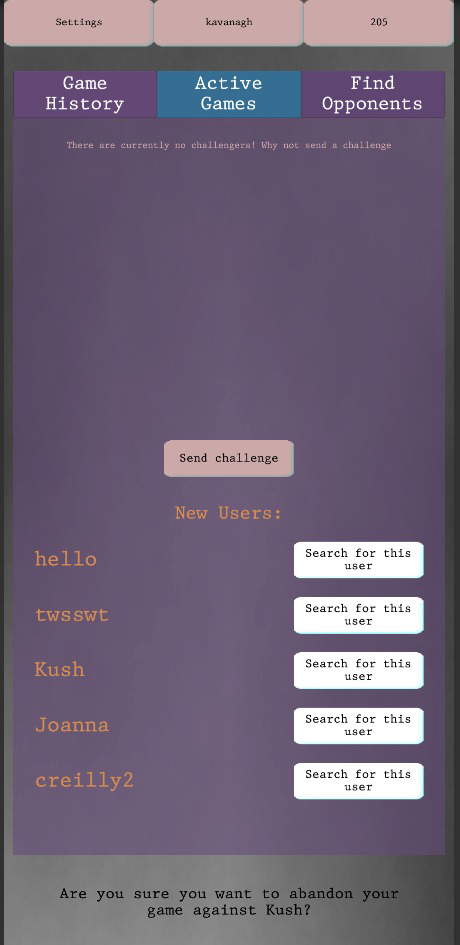
\includegraphics[width=.3\textwidth]{50_rpglite/images/find_users_1.jpeg}\hfill
    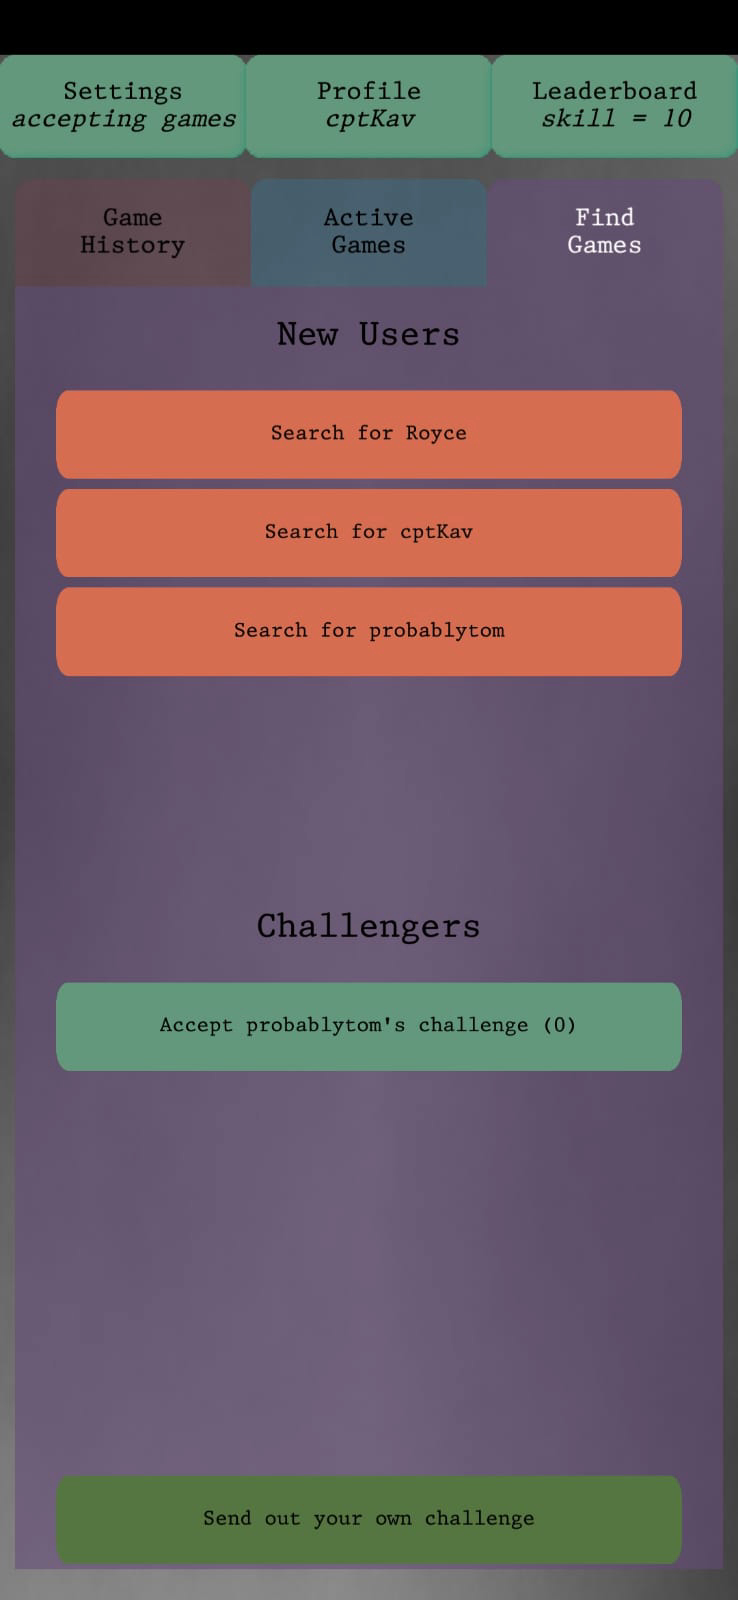
\includegraphics[width=.3\textwidth]{50_rpglite/images/find_users_2.jpeg}
    \caption{Evolution of the ``Find users'' matchmaking screen. Prototype left, final design right.}
    \label{fig:matchmaking_screen_improvements}
\end{figure}

\begin{figure}
    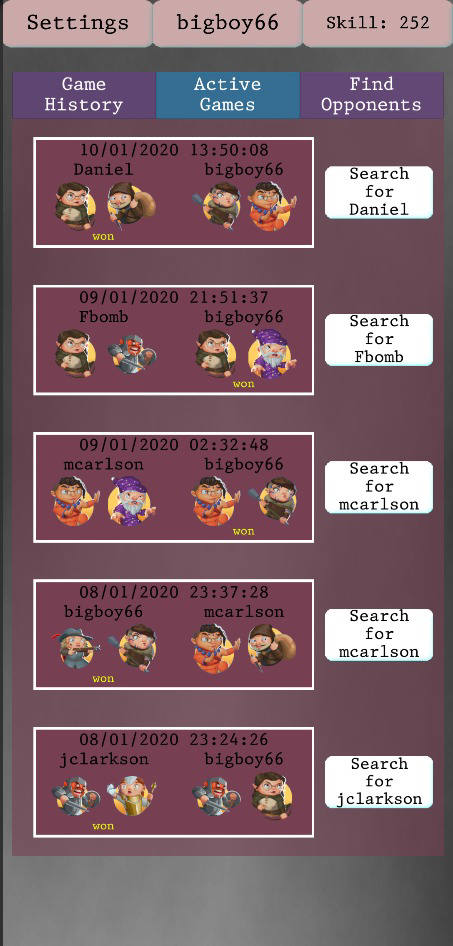
\includegraphics[width=.3\textwidth]{50_rpglite/images/homescreen_1.jpeg}\hfill
    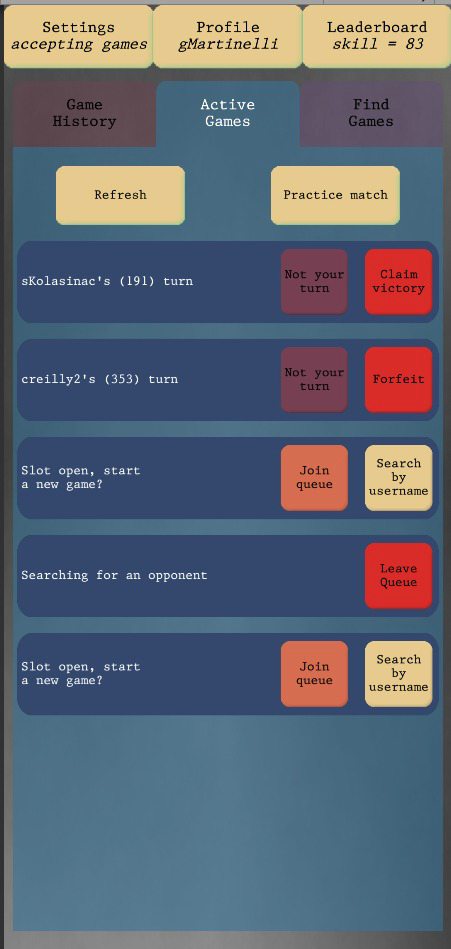
\includegraphics[width=.3\textwidth]{50_rpglite/images/homescreen_2.jpeg}\hfill
    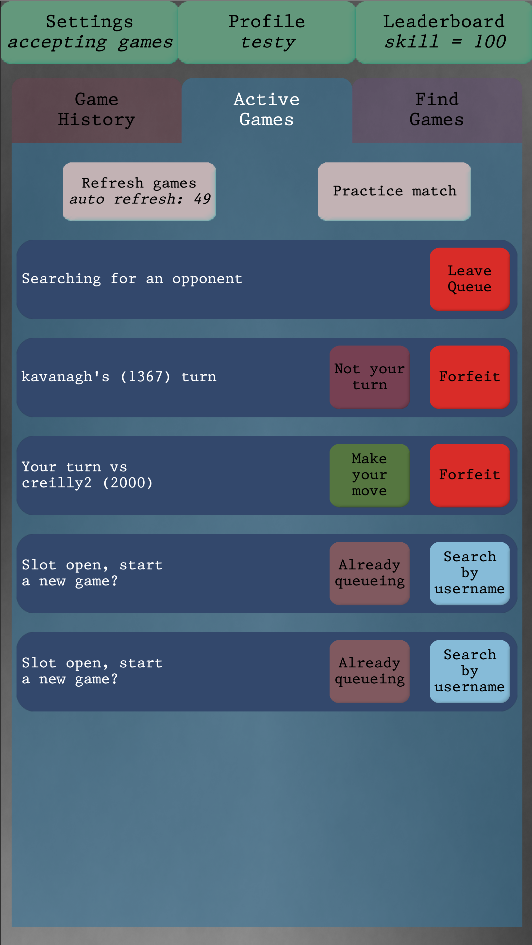
\includegraphics[width=.3\textwidth]{50_rpglite/images/homescreen_3.png}
    \caption{Evolution of the ``Active Games'' screen, which allowed RPGLite users to see and interact with games they were playing. An early prototype is shown to the left; a refinement through beta testing in the centre; and the final version released to the public to the right, with an improved colour palette.}
    \label{fig:homescreen_evolution}
\end{figure}

\begin{figure}
    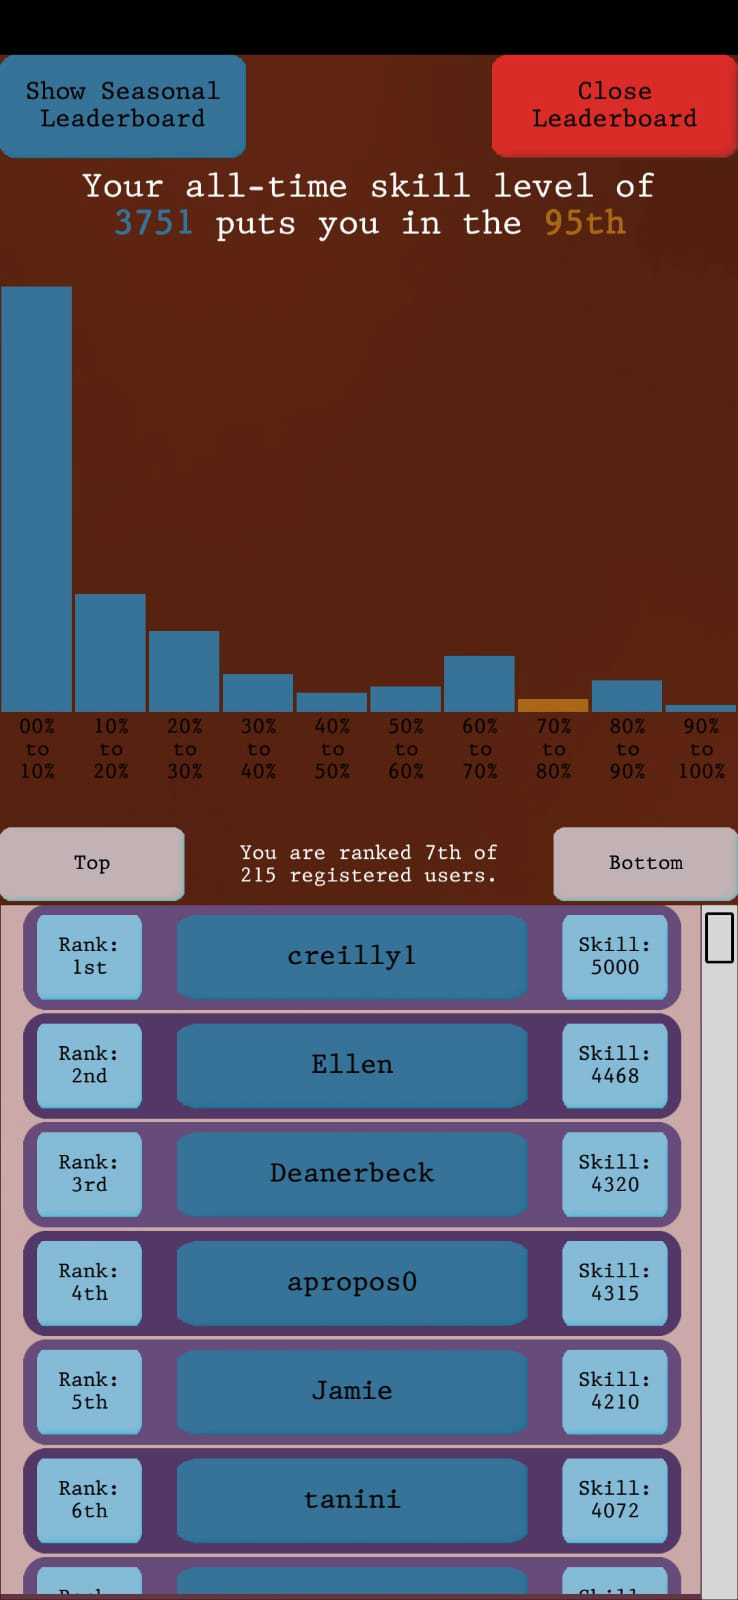
\includegraphics[width=.3\textwidth]{50_rpglite/images/leaderboard.jpeg}\hfill
    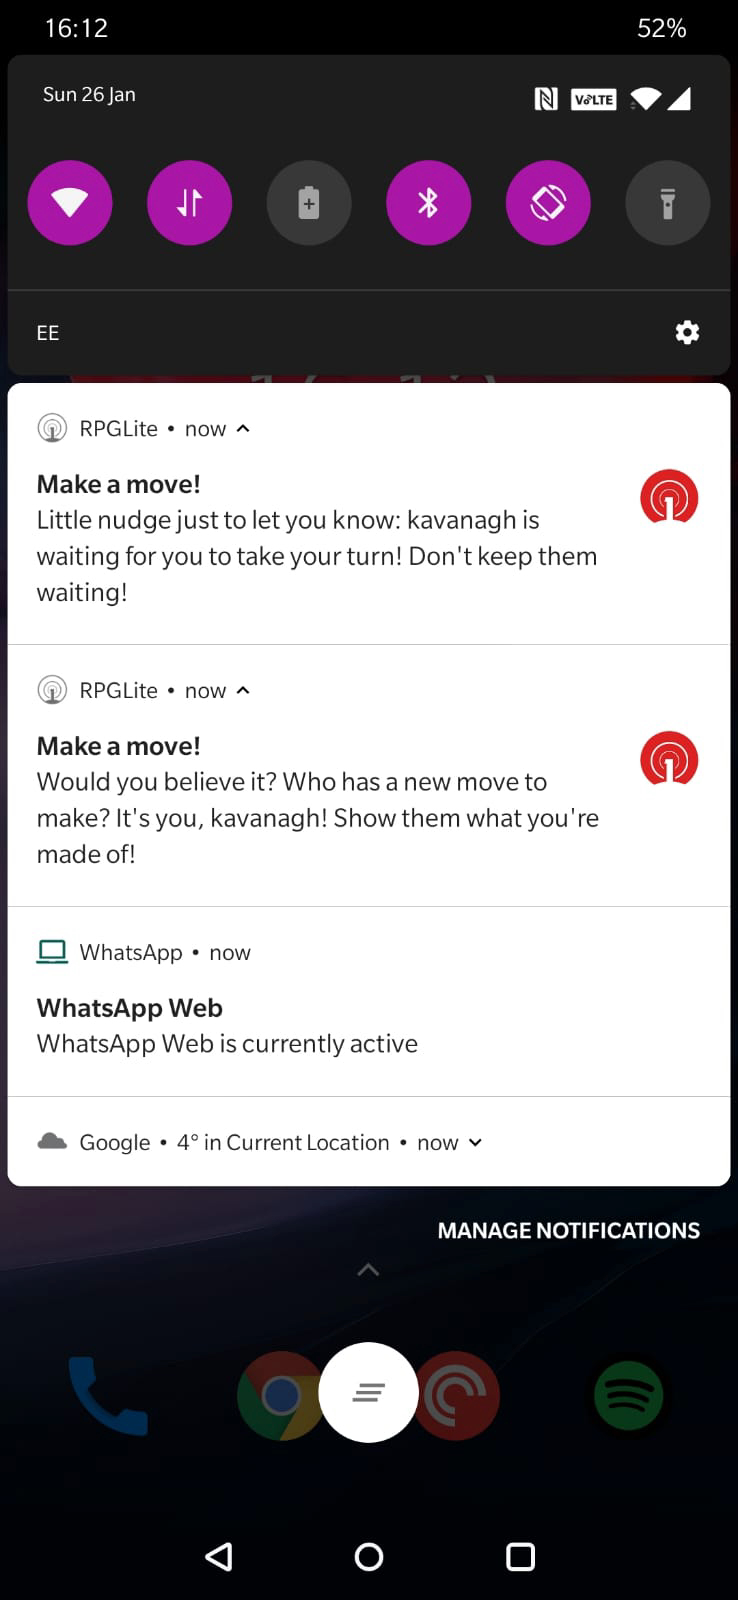
\includegraphics[width=.3\textwidth]{50_rpglite/images/notifications.jpeg}
    \caption{Features developed following requests from beta testers. A leaderboard of player engagement is shown to the left; examples of notifications when an opponent has acted are shown to the right.}
    \label{fig:extra_rpglite_features}
\end{figure}

\revnote{Attempt at subfigure layout given below, but it looks hideous and the old version's frankly better, so keeping it unless I have time to mess with the layouts.}

% \begin{figure}
%   \centering
%     \begin{subfigure}{0.3\textwidth}
%     \centering
%       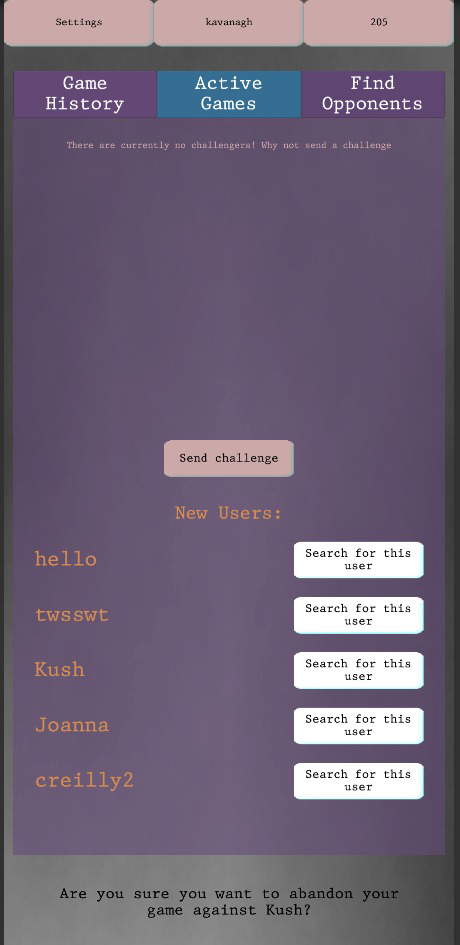
\includegraphics[width=\textwidth]{50_rpglite/images/find_users_1.jpeg}
%       \caption{Prototype matchmaking screen}
%     \end{subfigure}\hfill%
%     \begin{subfigure}{0.3\textwidth}
%     \centering
%       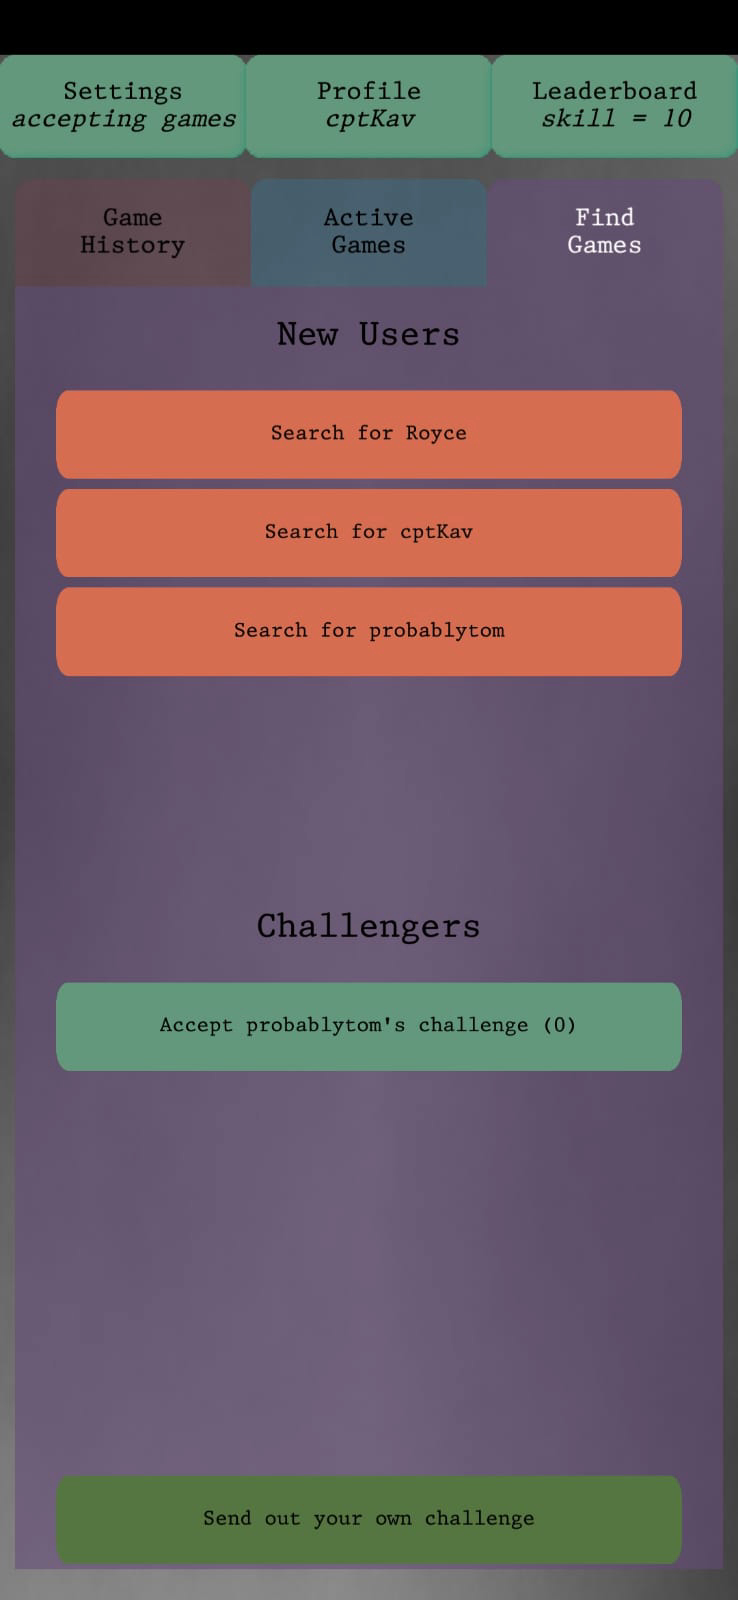
\includegraphics[width=\textwidth]{50_rpglite/images/find_users_2.jpeg}
%       \caption{Final matchmaking screen}
%     \end{subfigure}
%     \caption{Evolution of the ``Find users'' matchmaking screen's design}
%     \label{fig:matchmaking_screen_improvements}
% \end{figure}

% \begin{figure}
%   \centering
%   \begin{subfigure}{0.3\textwidth}
%     \centering
%     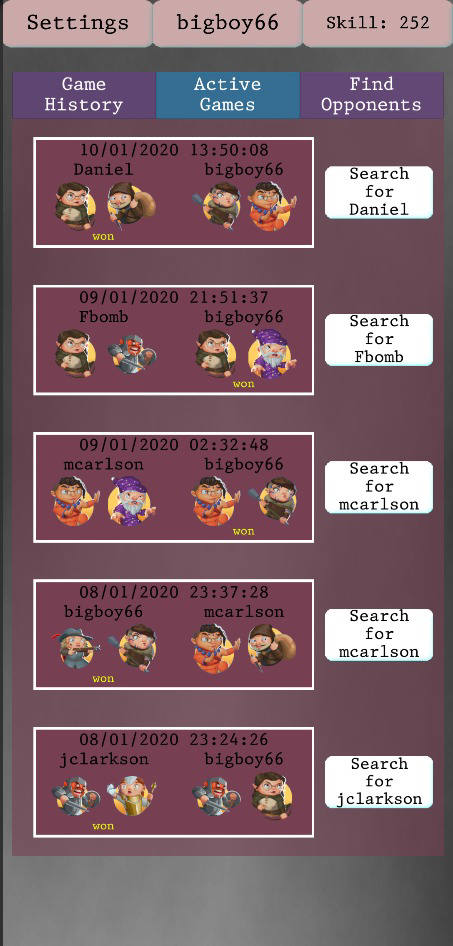
\includegraphics[width=\textwidth]{50_rpglite/images/homescreen_1.jpeg}\hfill
%     \caption{Early prototype ``Active games'' screen}
%   \end{subfigure}
%   \begin{subfigure}{0.3\textwidth}
%     \centering
%     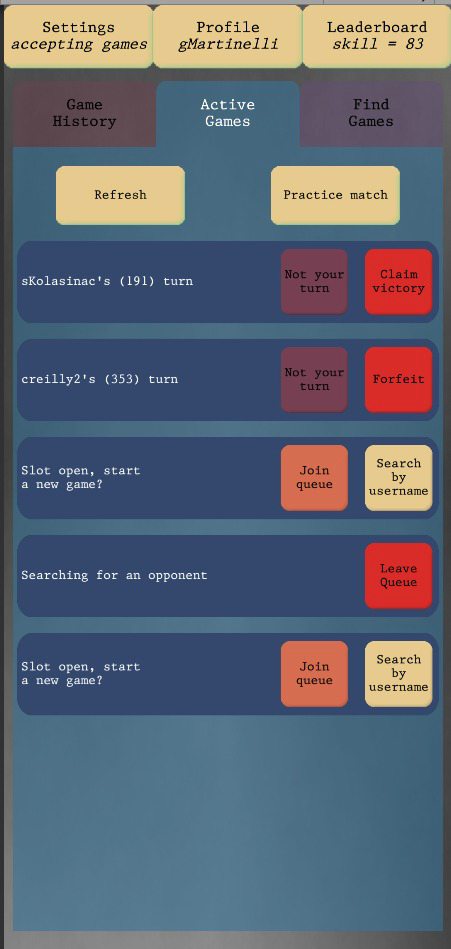
\includegraphics[width=\textwidth]{50_rpglite/images/homescreen_2.jpeg}\hfill
%     \caption{Refined ``Active games'' screen developed during beta testing with improved layout}
%   \end{subfigure}
%   \begin{subfigure}{0.3\textwidth}
%     \centering
%     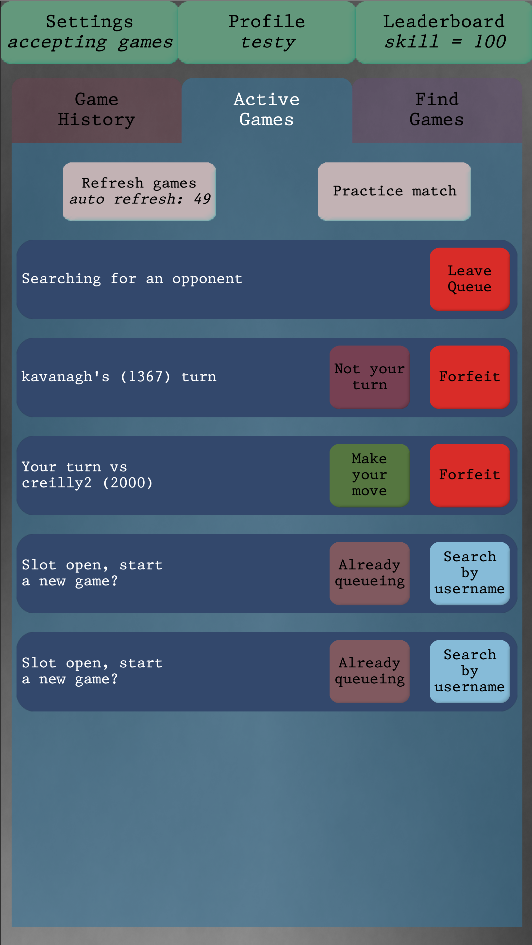
\includegraphics[width=\textwidth]{50_rpglite/images/homescreen_3.png}
%     \caption{Final ``Active games'' screen with improved colour palette}
%   \end{subfigure}
%   \caption{Evolution of the design of the ``Active Games'' screen, which allowed RPGLite users to see and interact with games they were playing.}
%   \label{fig:homescreen_evolution}
% \end{figure}

% \begin{figure}
%   \centering
%   \begin{subfigure}{0.3\textwidth}
%     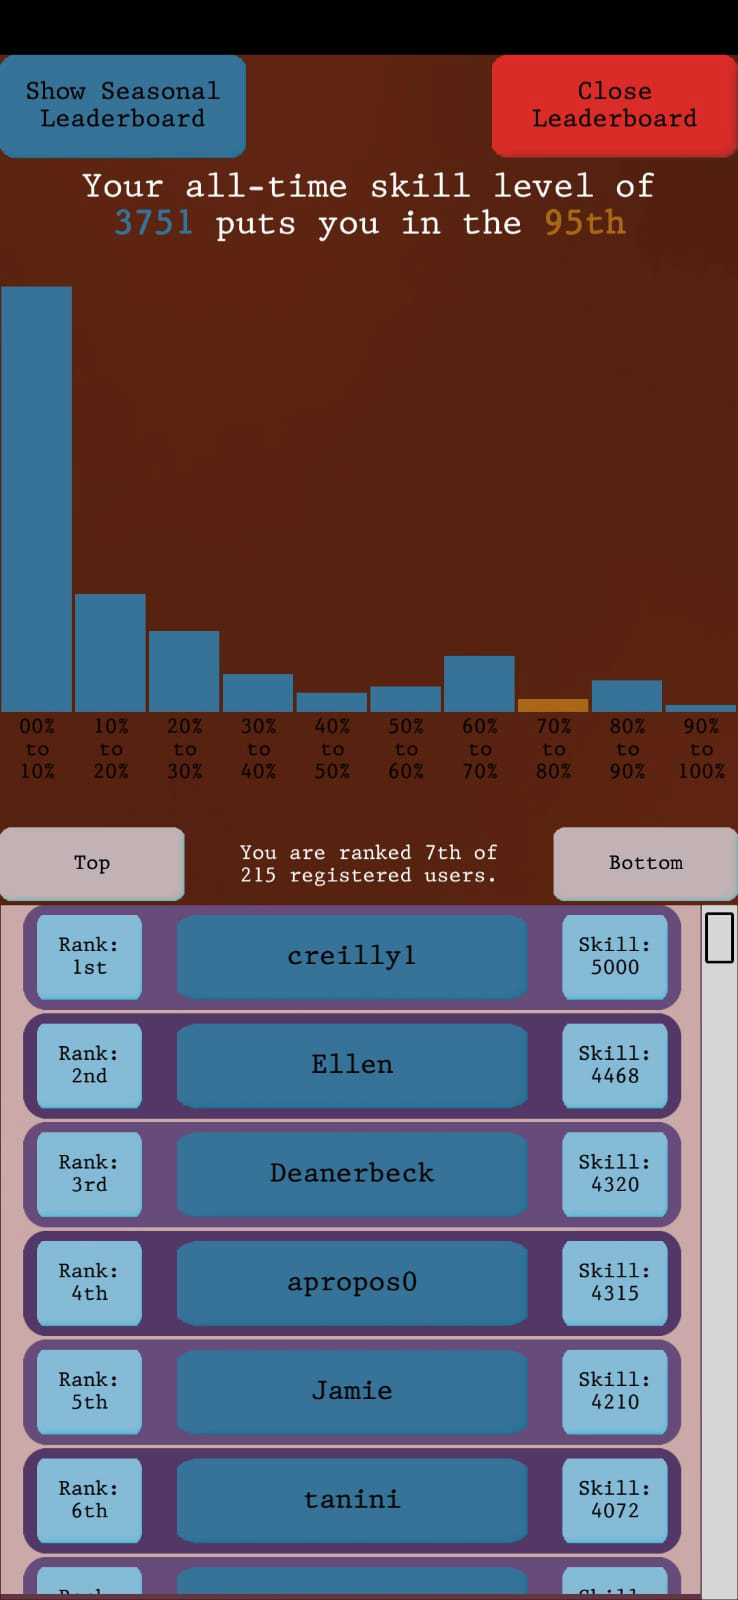
\includegraphics[width=\textwidth]{50_rpglite/images/leaderboard.jpeg}\hfill
%     \caption{Leaderboard of player engagement}
%   \end{subfigure}
%   \begin{subfigure}{0.3\textwidth}
%     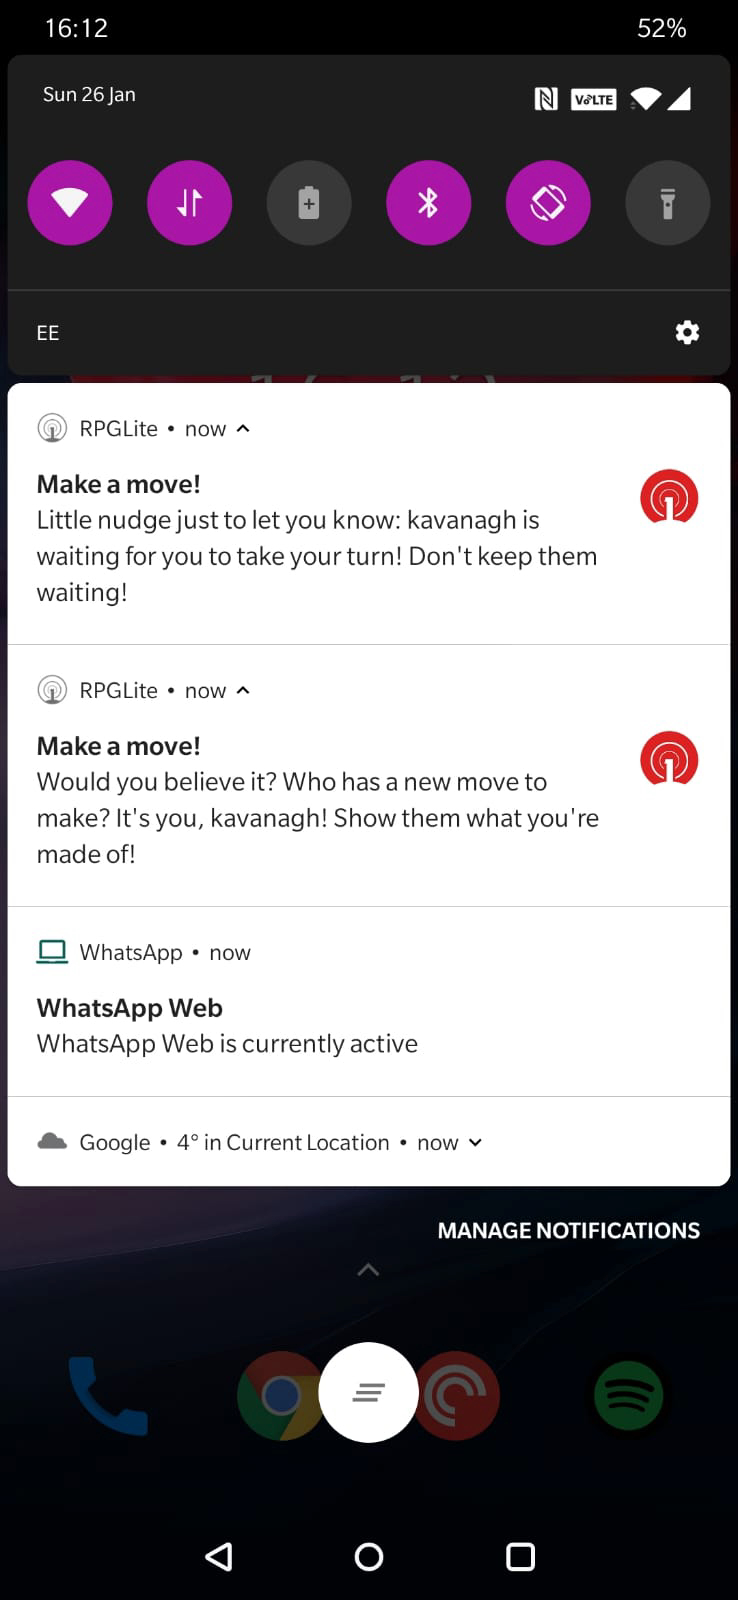
\includegraphics[width=\textwidth]{50_rpglite/images/notifications.jpeg}
%     \caption{Example notifications}
%   \end{subfigure}
%   \caption{Features developed following requests from beta testers. A leaderboard of player engagement is shown to the left; examples of notifications crawhen an opponent has acted are shown to the right.}
%   \label{fig:extra_rpglite_features}
% \end{figure}



An example of the game's visual evolution is given in
\cref{fig:matchmaking_screen_improvements}, where colourful buttons replace a
tabular, text-heavy interface. Another example is the evolution of the game's
main screen, ``Active Games'', which players were presented with upon logging
into the app and showed users active games they were involved in. The visual
identity and colour palette of this screen was refined iteratively, as can be
seen in \cref{fig:homescreen_evolution}. Other features which were developed
following feedback from beta testers include the implementation of a
notification system and a leaderboard showing a player's experience relative to
their peers. These are shown in \cref{fig:extra_rpglite_features}.
\revnote{There are some good screenshots in the paper for RPGLite; lessons
learned. Consider adding those here instead; the screenshots I've included at
present come from my iCloud photos library\ldots{}} 


\subsection{API \& Server-Side Logic}
\label{subsec:server-side-logic}

To develop the mobile game in such a way as to allow communication between two
RPGLite players remotely, a server and API for the game was required.

A REST API was developed with Python's \emph{Flask} framework. Endpoints were
created to support all in-game actions requiring centralised state (or a
recording of that state), allowing for player search, matchmaking, player
profile design, game history and statistics analysis, ranking calculations,
login and password reset, synchronisation of access to sensitive information,
and other in-game activities. The API also allowed moves to be made, and
rejected erroneous game states or unauthorised input from any malicious actor,
to ensure that the data collected, analysed, and published was not manipulated.
The API also sent push notifications to an opponent's device when moves were
made. This was a feature requested during beta testing, which was reported to
increase engagement with the game.

On each of these actions, data was collected about the action performed, and
logged in a database. In addition, in-game activities which required no
server-side input but were considered to have potential in later analysis would
log data points through the API into the same database.

A MongoDB database instance was installed and managed on a University of Glasgow
Computing Science virtual machine. The no-SQL nature of the database permitted
flexible structuring of the data, and simplified analysis of the games' results
after data collection was completed. The API was also hosted on the same virtual
machine. A combination of port access rules applied via Nginx and hardening the
security of the database itself through MongoDB's account features and
controlled permissions within the server prevented unauthorised access to the
database, ensuring that the data remained untampered.

Game state was initially interpreted client-side. The intention in this design
choice was to unburden a centralised service we were responsible for
maintaining, moving functionality such as calculating game states after moves
were created to clients on players' devices. This left the server-side logic
mostly concerned with executing database transactions and ensuring the integrity
of game states was uncompromised. However, some difficulties arose from this
decision: the lessons learned and corrective action taken are explained in
\cref{rpglite_lessons_learned_summary}.



\subsection{Player Recruitment \& Collection of Consent}
\label{subsec:consent_to_participation}

Players were recruited using a number of methods. Lecturers at the University of
Glasgow advertised the game to their students through email. Word of mouth was
used to advertise the game through our social and professional circles, and
contacts were encouraged to share the game in their own communities. The
Scottish branch of the International Game Developers Association advertised the
game to their group. A University of Glasgow newsletter for Science \&
Engineering undergraduate students was used to advertise the game.
\Cref{fig:rpglite_user_acquisition_over_time} shows player acquisition over
time. It is also reflected upon in
\cref{rpglite_lessons_learned_summary}
with regards the factors which impacted successful player recruitment. 

\begin{figure}
  \centering
  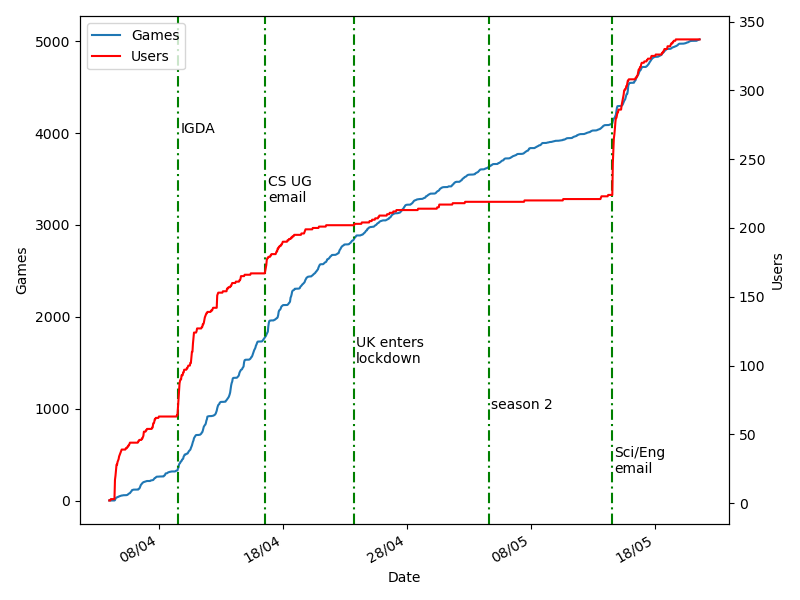
\includegraphics[width=0.8\textwidth]{50_rpglite/images/user_acquisition.png}
  \caption{Rate of user acquisition in the weeks following RPGLite's release.
  Important events are marked in the graph and include the promotion of the game
  via the Scottish branch of the International Game Developers Association, an
  email to Computing Science undergraduates at the University of Glasgow, the
  start of the UK's first COVID-19 lockdown, the release of a major update to
  RPGLite, and an email to all Science and Engineering undergraduates at the
  University of Glasgow.}
  \label{fig:rpglite_user_acquisition_over_time}
\end{figure}

Players gave consent to participate in a scientific study as a part of creating
an account to play RPGLite. Players were required to explicitly scroll through
an information sheet and consent agreement, and were required to agree to both
to make an account and play the game. Copies of both were made available to
download for player reference in both the game and RPGLite's
website~\cite{rpglite_website}. Players were instructed to contact the involved
researchers to withdraw participation, and were instructed that they could do so
at any time. Email addresses to contact were noted in both the app and on the
game's website~\cite{rpglite_website}.

The study, information sheet, consent form, and data collected were reviewed and
approved by the University of Glasgow Science \& Engineering ethics committee
before the game was released.


\subsection{Lessons Learned from RPGLite Implementation}
\label{rpglite_lessons_learned_summary}

Some observations were made about the mistakes made when producing RPGLite,
published separately to this thesis~\cite{RPGLiteLessonsLearned}. These were
documented to support other researchers in their own development processes who
were also new to game development, to avoid the need to ``learn the hard way''.

RPGLite's design was influenced heavily by beta testers, as mentioned in
\cref{rpglite_mobile_app}. Comments from beta testers formed a feedback loop
where rapid iteration on design and features could take place. This was
important because the game's release was timed to coincide with Glasgow
University's study break for exams, as students would have more time to play
when the teaching season ended and students were expected to constitute the
majority of RPGLite's community. Faster feedback from beta testers allowed for
quicker iterations on designs, and so allowed progress to be accelerated,
helping to meet the timeline originally agreed to. 


Recruitment of players was an important part of RPGLite's success, as a diverse
community of active players makes the published dataset more useful. The rate of
player acquisition and specific events expected to have influenced the game's
adoption is shown in \cref{fig:rpglite_user_acquisition_over_time}.

A lesson which was not immediately apparent when developing the game but is
significant in hindsight \revnote{too informal?} is that it was essential to make
use of our personal professional networks to advertise the game and build a
community. The game was shared by the chair of the Scottish branch of the
International Game Developers Association, which saw a large increase in player
count. The largest increase appears to have been advertising the game to all
Science \& Engineering students at the University of Glasgow. Other events were
expected to cause an increase in RPGLite's community: we believed that the UK
entering its first COVID-19 lockdown would encourage players to suggest the game
to their friends, but no significant increase in player account appears to have
been caused by this. The release of RPGLite's second season was also expected to
create some excitement in the community which might have encouraged the game to
be shared in players' social circles. However, no discernable increase in player
count appears to be attributable to the release of the new season. The most
significant factor in RPGLite's accumulation of players therefore appears to be
active promotion through our available networks, rather than players promoting
the game within their own social circles.

RPGLite was designed to validate game state client-side, and used the server it
communicated with largely as a mechanism to communicate updates to game state.
This minimised the work involved in developing RPGLite's server and API.
However, the Unity-based mobile game proved more difficult to debug than the
Python-based server, and logic was duplicated across both codebases as the
server had to validate game state --- a task originally intended for the mobile
client --- to prevent players cheating by crafting requests to the server which
would update a game with an inauthentic state. Updates to the server were also
easier to control than updates to the mobile game, as deploying a new version of
the server was simple but deploying a new version of the app required all
players to update, which was outwith our control as developers. As the server
was ultimately responsible for RPGLite's security, had to include all game
logic, was easier to develop than the mobile game, and additions to the game
were more easily deployed through the server than through the mobile client,
development effort shifted toward the server and away from the mobile client as
we gained real-world experience in developing mobile games. \revnote{I use
``we'' in this para. Couldn't avoid it. I try not to use it throughout the
thesis though. Can I rephrase?}



\subsection{RPGLite Seasons}
\label{seasons_of_rpglite}
\label{rpglite_configurations}

RPGLite was played through two ``seasons'': after an initial 3,000 games
played, the game was updated and a second configuration was released. This meant
that, having learned a strategy to play with the initial configuration (such as
a preference of characters) changes were made which may invalidate what players
had learned. The dataset therefore contains two conceptual subsets: data
collected from a system with the same mechanics but tweaked parameters,
resulting in different optimal character pairs and moves. Parameters for
characters in season 1 are given in \cref{fig:s1_config}, in
\cref{fig:s2_config} for season 2, and the differences between the two
configurations are summarised in \cref{fig:changes_between_seasons}.

\begin{table}[h]
  \begin{minipage}{.50\columnwidth}
    \centering
    \begin{tabular}{@{}l r r r@{}}
      \toprule
      \emph{Character} & \emph{Health} & \emph{Hit Accuracy} & \emph{Damage}\\
      \midrule
      Knight & 10 & 0.60 & 4 \\
      Archer & 8 & 0.85 & 2 \\
      Wizard & 8 & 0.50 & 2 \\
      Rogue & 8 & 0.75 & 3 \\
      Healer & 10 & 0.85 & 2 \\
      Barbarian & 10 & 0.75 & 3 \\
      Monk & 7 & 0.80 & 1 \\
      Gunner & 8 & 0.80 & 4 \\
      \bottomrule
    \end{tabular}
    \caption{Configuration for RPGLite\\in season 1.}
    \label{fig:s1_config}
  \end{minipage}%
  \begin{minipage}{.50\columnwidth}
    \centering
    \begin{tabular}{@{}l r r r@{}}
      \toprule
      \emph{Character} & \emph{Health} & \emph{Hit Accuracy} & \emph{Damage}\\
      \midrule
      Knight & 10 & 0.80 & 3 \\
      Archer & 8 & 0.85 & 2 \\
      Wizard & 8 & 0.50 & 2 \\
      Rogue & 8 & 0.70 & 3 \\
      Healer & 9 & 0.90 & 2 \\
      Barbarian & 9 & 0.70 & 3 \\
      Monk & 7 & 0.75 & 1 \\
      Gunner & 8 & 0.70 & 4 \\
      \bottomrule
    \end{tabular}
    \caption{Configuration for RPGLite\\in season 2.}
    \label{fig:s2_config}
  \end{minipage}
\label{fig:table_of_char_params_between_seasons}
\end{table}

In the second configuration, most character pairs have their hit accuracy
reduced by 0.05 percentage points. Only the knight's damage is reduced, from 4
points to 3. Health is set to 9 for the Archer, Healer, and Barbarian. This
change alters RPGLite's metagame, as making certain characters weaker and others
stronger incentivises different strategies of play: different character pairs
and moves are optimal as a result of the changed configuration. Player response
to changed configuration is analysed using formal methods by
\citet{kavanagh2021thesis}.
\revnote{
  Ideally we'd say a little more about RPGLite's two seasons, but I'm not sure
  exactly what to say. We've got the important details here. Expand if there's
  time; if there's not, that's OK, add more before the viva.
}


\begin{table}[h]
  \centering
  \begin{tabular}{@{}l l r r@{}@{}}
    \toprule
    \emph{Parameter} & \emph{Character} & \emph{Old Value} & \emph{New Value} \\
    \midrule
    \multirow{7}{*}{Hit Accuracy} & Knight    & 0.60 & 0.80 \\
                                  & Archer    & 0.85 & 0.80 \\
                                  & Rogue     & 0.75 & 0.70 \\
                                  & Healer    & 0.85 & 0.90 \\
                                  & Barbarian & 0.75 & 0.70 \\
                                  & Monk      & 0.80 & 0.75 \\
                                  & Gunner    & 0.75 & 0.70 \\
    \midrule
    \multirow{1}{*}{Damage}       & Knight    & 4    & 3    \\
    \midrule
    \multirow{3}{*}{Health}       & Archer    & 8    & 9    \\
                                  & Healer    & 10   & 9    \\
                                  & Barbarian & 10   & 9    \\
    \bottomrule
  \end{tabular}
  \caption{Altered values of different parameters when moving from season 1 to season 2.}
  \label{fig:changes_between_seasons}
\end{table}


\subsection{Data Collected}
\label{sec:rpglite_data_discussed}

In total, 360 players produced a dataset of 9,323 games, 170 of which were in
progress when the dataset was created from a snapshot of the MongoDB database
used to develop the game. This snapshot was taken in November 2020, around 8
months after the game was initially released. The dataset includes 1,069,595
data points generated by gameplay or player interaction with the client, such as
players checking their position on a leaderboard, searching their game history,
or rolling to hit as part of an attack. These data points are ancillary to the
games themselves and mostly record interactions players made with the mobile
game. These were initially collected for diagnostic purposes, but were published
as part of the dataset to support future research, should they be useful for
other research projects.

This data is published and available in the format of a JSON
object~\cite{rpglite_dataset}. The object has three attributes:
\lstinline{"games"}, which contains a record of the 9,323 games played by
RPGLite players;  \lstinline{"page_hits"}, containing data points describing
interactions with the RPGLite app; and \lstinline{"players"}, which contains
every username registered to play RPGLite.

The \lstinline{"players"} attribute of the dataset contains only a list of
usernames, represented as strings.

The \lstinline{"page_hits"} attribute contains a list of ``page hit'' objects.
The ``page hit'' name for these attributes is a historical artefact of the
game's development, and --- while esoteric --- is not a description of the data
itself, which mostly concerns app interaction. The specific interaction
described by each data point (rather than the history of a specific game) is
denoted by a ``kind'' field within each data point. 63 such kinds are included in
the dataset. Some examples are described in \cref{fig:page_hit_datapoint_examples}.

\begin{table}
  \centering
\begin{tabular}{@{}lp{0.45\textwidth}r@{}}
\toprule{}
\begin{tabular}{@{}l@{}}\emph{String identifier}\\\emph{for ``kind''}\end{tabular} &
\emph{Contents of data point specified by ``kind''} &
\emph{\# data points} \\
\midrule{}
\lstinline[]$rolls_fastforwarded$ & Player fast-forwarded the animation of a roll
determining the outcome of an attack & 187,797 \\
\rule{0pt}{2em}\lstinline[]$home_to_gameplay$ & Player viewed a game from their home screen &
100,071 \\
\rule{0pt}{2em}\lstinline[]$hs_refresh_pressed$ & Player refreshed their list of active games to
check for updates & 24,798 \\
\rule{0pt}{2em}\lstinline[]$tabbed_to_find_opponents$ & Player used the ``Find games'' tab to find a
new opponent to challenge to a game & 15,531 \\
\rule{0pt}{2em}\lstinline[]$homescreen_to_leaderboard$ & Player moved from their
home screen to
the game's leaderboard & 7,394 \\
\rule{0pt}{2em}\lstinline[]$homescreen_to_profile$ & Player checked their own profile from their
home screen & 3,005 \\
\rule{0pt}{2em}\lstinline[]$game_abandoned$ & Player abandoned a game & 2,018 \\
\rule{0pt}{2em}\lstinline[]$leaderboard_user_zoom$ & Player investigated another player
discovered from the leaderboard & 1,385 \\
\rule{0pt}{2em}\lstinline[]$challenge_sent$ & User challenged another user to a game & 1,291 \\
\rule{0pt}{2em}\lstinline[]$customise_tag$ & User customised the tag displaying their username in
a game & 114 \\
\rule{0pt}{2em}\lstinline[]$notifications_toggled$ & User toggled notifications on or off & 71 \\
\bottomrule{}
\end{tabular}
\caption{Some types of data included in the 1,069,595 ``page hit'' data points, which mostly describe interactions with the RPGLite app.}
\label{fig:page_hit_datapoint_examples}
\end{table}

The abridged list of different page hit data points described in
\cref{fig:page_hit_datapoint_examples} contains some kinds of particular
interest. Refreshing the list of games on the home screen occurred frequently:
with 24,798 data points logged, it was the eight most common interaction with
the game. This is surprising, as the list of games refreshed automatically when
game states changed (i.e. when an opponent made a move), and players were sent
notifications if they were not logged into the game. Future research could
investigate whether players who checked on their games' statuses were
particularly likely to engage with RPGLite for a long period of time, or whether
engagement with their list of games correlates with a player's degree of optimal
play. These events also reveal information about how players engaged with the
application's features: players moved to the ``Find games'' tab around twice as
often as they moved to the leaderboard. Notifications were toggled only 71
times, meaning that a maximum of 19.72\% of players could have disabled their
notifications, which were on by default. As some players likely re-enabled
notifications, the proportion is expected to be lower than this estimate. This
either implies that most players did not mind receiving notifications from
RPGLite, or that they managed their notifications some other way (such as
through their phones' operating system settings) or did not play enough to
notice the notifications. More investigation is required to determine insights
about RPGLite's community and their interactions with the application from these
data points.

Finally, the \lstinline{"games"} attribute of the RPGLite dataset contains a
list of JSON objects describing the state of a game. Each object contains
similar attributes describing the entire history of the RPGLite game played;
attributes of particular interest are highlighted in
\cref{fig:gamedoc_attributes}. 

\begin{table}
  \centering
  \begin{tabular}{@{}lp{0.73\textwidth}@{}}
    \toprule{}
    \emph{Attribute} & \emph{Description of attribute}\\
    \midrule{}
    \rule{0pt}{2em}\lstinline[]$usernames$ & A list of usernames for the players in the game\\
    \rule{0pt}{2em}\lstinline[]$winner$ & Only exists for completed games. A number indicating
    which user in the list of usernames won the game, where 1 is the first
    username and 2 is the second. \\
    \rule{0pt}{2em}\lstinline[]$Moves$ & A list of moves made in the game. Moves are written in
   a chess-like notation explained in \cref{sec:rpglite_data_discussed}. \\
    \rule{0pt}{2em}\lstinline[]$p1c1$ & Player 1's first selected character \\
    \rule{0pt}{2em}\lstinline[]$p1c2$ & Player 1's second selected character \\
    \rule{0pt}{2em}\lstinline[]$p2c1$ & Player 2's first selected character  \\
    \rule{0pt}{2em}\lstinline[]$p2c2$ & Player 2's second selected character  \\
    \rule{0pt}{2em}\lstinline[]$p1_abandon$ & A boolean representing whether p1 forfeited the game \\
    \rule{0pt}{2em}\lstinline[]$p2_abandon$ & A boolean representing whether p2 forfeited the game \\
    \rule{0pt}{2em}\lstinline[]$elo_scores_at_end$ & A mapping of usernames to floating point
    ELO scores, a player ranking metric common in games like Chess~\cite{elo_ratings} \\
    \rule{0pt}{2em}\lstinline[]$balance_code$ & A string value identifying the RPGLite
    configuration (or ``season'') the game refers to. Season 1 games have no
    such attribute, and so are identified by the lack of a balance code. Season
    2 games have the balance code \lstinline[]$"1.2"$. No other seasons of
    RPGLite were released.\\
    \bottomrule{}
  \end{tabular}
  \caption{Examples of attributes common to records of RPGLite games as published in the RPGLite gameplay dataset~\cite{rpglite_dataset}.}
  \label{fig:gamedoc_attributes}
\end{table}

Moves stored in game objects are encoded in a string format similar to chess
move notation. A move notated as \lstinline{p1Gp2A_65} reads as, \emph{``Player
1's Gunner attacked Player 2's Archer, rolling a 65 to hit''}. Values for rolls
range from 1 to 100 and are compared against the attacking character's chance to
hit in the configuration being used to determine whether the attack is
successful: an attack is a success if $roll > 1 - (acc \times 100)$, where
$roll$ is the value rolled to hit and $acc$ is the accuracy of the attacking
character. The notation is composed of the following segments: 

\medskip{}
{\centering

  \begin{tabular}{cccccc}
    \begin{tabular}{@{}c@{}}Active\\Player\end{tabular} & 
    \begin{tabular}{@{}c@{}}Attacking\\Character\end{tabular} &
    \begin{tabular}{@{}c@{}}~\\Opponent\end{tabular} &
    \begin{tabular}{@{}c@{}}Opponent's Targeted\\Character\end{tabular} &
    ~ &
    \begin{tabular}{@{}c@{}}Roll\\To Hit\end{tabular} \tabularnewline{}
    p1 & G & p2 & A & \_ & 65\\
  \end{tabular}

}

The Healer and Archer characters produce variations on this notation due to
their special abilities. The notation is extended in each case. The Archer can
attack two characters when they move, and rolls for each target must be
recorded. An example of the notation describing each of an Archer's rolls is
\lstinline{p2Ap1G_41p1R_25}, which reads similarly to the original example, but
contains a second target at the end. The healer includes both the targeted
opponent character to deal damage to and the character belonging to the
attacking player which the Healer will heal if the attack is successful. An
example of the Healer's notation is \lstinline{p2Hp1Gp2A_48}, which describes a
Healer attacking an opponent Gunner and healing the active character's Archer.
The notation extends similarly for other characters.

\section{Discussion}
\label{rpglite_discussion_section}

A mobile game, RPGLite, was implemented and distributed to collect data for
research purposes. It followed an existing game design to support formal
analysis through model checking~\cite{kavanagh2019balancing}. The dataset
produced by the game~\cite{rpglite_dataset} was released to the public after
around 8 months of play from 360 players who participated in 9,323 games.
Players were recruited using the University of Glasgow's outreach channels to
advertise the game to undergraduate students in particular. The data collected
from these players' games and interactions with the application include specific
moves made within games, the characters chosen, players' use of application
features such as its leaderboard and challenge system, and players' ELO ratings
(a popular metric to rank players of games, originating in chess~\cite{elo_ratings}).

Aside from the dataset produced from the game, the technical contribution to the
game's implementation which is attributable to this thesis is its server-side
component and networking. Management of the game's hosting was also contributed.
The dataset forms the foundation of the experiments discussed in
\cref{chap:experiment_setup} and \cref{chap:experimental_results}, and is hoped
to support other research in the future. Some reflections on the development
process were written and published to assist other researchers who must also
develop mobile games for research purposes~\cite{RPGLiteLessonsLearned}, some of
which were summarised in \cref{rpglite_lessons_learned_summary}.
